Para $\mathbf{F}(x,y)=\langle-y,x\rangle$, construya una parametrización por tramos de la trayectoria cerrada mostrada y calcule $\oint_C\mathbf{F}\cdot d\vec r$.
\begingroup
\shorthandoff{>}
\begin{center}
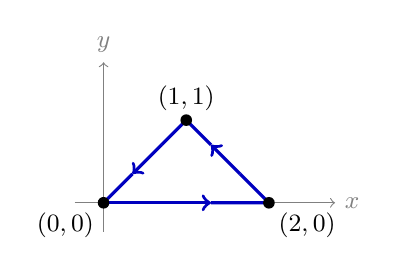
\begin{tikzpicture}[scale=1.05,every node/.style={font=\small}]
    \draw[->,gray] (-.35,0)--(2.8,0) node[right] {$x$};
    \draw[->,gray] (0,-.35)--(0,1.7) node[above] {$y$};
    \draw[blue!75!black,very thick,->] (0,0)--(1.3,0);
    \draw[blue!75!black,very thick] (1.3,0)--(2,0)--(1.65,.35);
    \draw[blue!75!black,very thick,->] (1.65,.35)--(1.3,.7);
    \draw[blue!75!black,very thick] (1.3,.7)--(1,1)--(.7,.7);
    \draw[blue!75!black,very thick,->] (.7,.7)--(.35,.35);
    \draw[blue!75!black,very thick] (.35,.35)--(0,0);
    \fill (0,0) circle (2pt) node[below left] {$(0,0)$};
    \fill (2,0) circle (2pt) node[below right] {$(2,0)$};
    \fill (1,1) circle (2pt) node[above] {$(1,1)$};
\end{tikzpicture}
\end{center}
\endgroup
